% GENERATED by implementation/experiments/scripts/render_v005_supplement.py.
% Do not edit by hand -- regenerate from results/runs/<root>/analysis/ instead.
\begin{table*}[t]
    \centering
    \footnotesize
    \setlength{\tabcolsep}{2pt}
    \caption{Cost to target (pre-registration \S5.2), $b = 350$: median number of full evaluations (MF arms: cost in full-evaluation equivalents) after which a run first reaches 90, 95 or 99\,\% of the best median final quality in the cell (HV: $q \cdot$ best; IGD+: best$/q$), over the runs that reach it; in brackets the percentage of the 30 runs that do, when below 100; -- = no run does. Simulated training time to target is in the released \texttt{cost\_to\_target.csv}.}
    \label{tab:v005-s-ctt}
    \begin{tabular}{@{}lrrrrrrrrrrrr@{}}
        \toprule
        & \multicolumn{3}{c}{C10} & \multicolumn{3}{c}{CRC} & \multicolumn{3}{c}{FMN} & \multicolumn{3}{c}{NHB} \\
        \cmidrule(lr){2-4}\cmidrule(lr){5-7}\cmidrule(lr){8-10}\cmidrule(lr){11-13}
        \textbf{Arm} & 90\,\% & 95\,\% & 99\,\% & 90\,\% & 95\,\% & 99\,\% & 90\,\% & 95\,\% & 99\,\% & 90\,\% & 95\,\% & 99\,\% \\
        \midrule
        P3Net & 24 & 32 & 124\,(67) & 22 & 23 & 135\,(87) & 18 & 18 & 127\,(90) & 282\,(3) & 284\,(3) & 300\,(3) \\
        \midrule
        P3 (canonical) & 32 & 38 & 143\,(70) & 24 & 28 & 106\,(87) & 28 & 28 & 112\,(87) & -- & -- & -- \\
        P3Net-gate & 24 & 32 & 123\,(63) & 22 & 23 & 135\,(87) & 18 & 18 & 127\,(90) & 285\,(3) & 287\,(3) & 303\,(3) \\
        P3Net-nolink & 24 & 32 & 124\,(67) & 22 & 23 & 135\,(87) & 18 & 18 & 127\,(90) & 282\,(3) & 284\,(3) & 300\,(3) \\
        P3-eLyMPuS & 32 & 38 & 139\,(67) & 24 & 28 & 139\,(87) & 28 & 28 & 116\,(90) & -- & -- & -- \\
        \midrule
        MO-DSA & 4 & 10 & 74\,(37) & 3 & 6 & 70\,(97) & 3 & 3 & 19\,(97) & 288\,(7) & 320\,(3) & 320\,(3) \\
        MO-PSA & 4 & 10 & 155\,(70) & 3 & 6 & 70 & 3 & 3 & 20 & -- & -- & -- \\
        NSGA-Net & 4 & 10 & 105\,(97) & 3 & 6 & 72 & 3 & 3 & 20 & 305\,(20) & 305\,(17) & 292\,(10) \\
        NSGANetV2 & 4 & 10 & 106 & 3 & 6 & 73 & 3 & 3 & 20 & 274\,(50) & 276\,(50) & 282\,(50) \\
        REINFORCE & 4 & 8 & 64\,(20) & 3 & 5 & 43\,(43) & 2 & 4 & 17\,(70) & -- & -- & -- \\
        RegEvo & 4 & 10 & 90\,(97) & 3 & 6 & 62 & 3 & 3 & 20 & 295\,(17) & 295\,(17) & 302\,(13) \\
        MO-LS & 24 & 32 & 88 & 22 & 25 & 66 & 22 & 22 & 37 & -- & -- & -- \\
        SH-EMOA & 4 & 10 & 86 & 3 & 6 & 48 & 3 & 3 & 20 & 267\,(23) & 276\,(23) & 305\,(17) \\
        NSGA-III & 4 & 10 & 96 & 3 & 6 & 62 & 3 & 4 & 20 & 340\,(20) & 299\,(10) & 309\,(10) \\
        MOEA/D & 4 & 10 & 216\,(73) & 3 & 6 & 89 & 3 & 3 & 20 & 341\,(3) & 341\,(3) & 341\,(3) \\
        MO-BANANAS & 4 & 10 & 86 & 3 & 6 & 50 & 3 & 4 & 22 & 307\,(10) & 338\,(7) & -- \\
        MOTPE & 4 & 10 & 76\,(97) & 3 & 6 & 43\,(97) & 3 & 4 & 18 & 321\,(3) & 324\,(3) & 350\,(3) \\
        SMAC3-ParEGO & 4 & 10 & 130 & 3 & 7 & 80 & 3 & 4 & 19 & 305\,(3) & 305\,(3) & 305\,(3) \\
        Random search & 4 & 10 & 208\,(93) & 3 & 6 & 73 & 3 & 3 & 20 & -- & -- & -- \\
        Hyperband & 7 & 14 & 248\,(83) & 7 & 10 & 61 & 4 & 4 & 19 & -- & -- & -- \\
        ASHA & 7 & 9 & 82 & 7 & 7 & 19 & 4 & 5 & 10 & -- & -- & -- \\
        SH-EMOA (MF) & 231 & 231 & 236 & 231 & 231 & 231 & 231 & 231 & 234 & 327\,(13) & 318\,(10) & 317\,(7) \\
        \midrule
        MOSH-BANANAS & 7 & 10 & 175\,(80) & 4 & 7 & 51 & 4 & 5 & 28 & -- & -- & -- \\
        MO-BOHB & 7 & 10 & 100 & 4 & 7 & 60 & 4 & 5 & 21 & 329\,(3) & 329\,(3) & 329\,(3) \\
        \bottomrule
    \end{tabular}
\end{table*}


\begin{table*}[t]
    \centering
    \footnotesize
    \setlength{\tabcolsep}{2pt}
    \caption{Budget use (pre-registration \S5.7), all spaces and budgets: arms whose runs do not all end by exhausting the budget (5 of 27; every other arm exhausts it in every run). The share of re-proposed solutions recorded in the run records is 0 for every run, because duplicates are filtered before evaluation and cost no budget (decision \#35); re-proposal shows only as the stop reasons below.}
    \label{tab:v005-s-budget}
    \begin{tabular}{@{}lrrp{0.55\textwidth}@{}}
        \toprule
        \textbf{Arm} & \textbf{Runs} & \textbf{Runs exhausting the budget, \%} & \textbf{Other stop reason} \\
        \midrule
        MO-DSA & 1\,080 & 80.9 & exploration collapse: 1000 iterations without a new real evaluation \\
        MO-PSA & 1\,080 & 88.0 & exploration collapse: 1000 iterations without a new real evaluation \\
        REINFORCE & 1\,080 & 15.8 & exploration collapse: 10000 consecutive duplicate samples (\#36) \\
        MOTPE & 1\,080 & 99.6 & exploration collapse: 10000 asks without a new genotype \\
        SH-EMOA (MF) & 960 & 0.0 & algorithm finished \\
        \bottomrule
    \end{tabular}
\end{table*}


\begin{table*}[t]
    \centering
    \footnotesize
    \setlength{\tabcolsep}{2pt}
    \caption{HV sensitivity to the reference point (pre-registration \S5.6a), JAHS-Bench-201: Spearman correlation of the order of arms by median HV at reference points $(1.05, 1.05)$ and $(1.2, 1.2)$ with the order at the primary $(1.1, 1.1)$, and P3Net's rank at each (ties share the lower rank). Medians per arm and cell are in the released \texttt{hv\_sensitivity.csv}.}
    \label{tab:v005-s-hvsens}
    \begin{tabular}{@{}lrrrrrrr@{}}
        \toprule
        \textbf{Space} & \textbf{$b$} & $\rho_{1.05}$ & $\rho_{1.2}$ & \multicolumn{3}{c}{P3Net rank at 1.05 / 1.1 / 1.2} & \textbf{Arms} \\
        \midrule
        C10 & 50 & 0.996 & 0.999 & 26 & 26 & 26 & 27 \\
        C10 & 100 & 0.999 & 0.999 & 23 & 23 & 23 & 27 \\
        C10 & 200 & 0.999 & 0.998 & 22 & 22 & 22 & 24 \\
        C10 & 350 & 1.000 & 0.997 & 9.5 & 9.5 & 9.5 & 24 \\
        CRC & 50 & 0.999 & 0.998 & 24 & 24 & 24 & 27 \\
        CRC & 100 & 1.000 & 0.999 & 25 & 25 & 25 & 27 \\
        CRC & 200 & 0.998 & 0.999 & 2 & 2 & 2 & 24 \\
        CRC & 350 & 1.000 & 1.000 & 6 & 6 & 6 & 24 \\
        FMN & 50 & 0.999 & 0.992 & 26 & 26 & 26 & 27 \\
        FMN & 100 & 1.000 & 0.999 & 26 & 26 & 26 & 27 \\
        FMN & 200 & 1.000 & 0.998 & 3 & 3 & 3 & 24 \\
        FMN & 350 & 0.999 & 0.998 & 3 & 3 & 3 & 24 \\
        \bottomrule
    \end{tabular}
\end{table*}


\begin{table*}[t]
    \centering
    \footnotesize
    \setlength{\tabcolsep}{2pt}
    \caption{Simple regret of $f_1$ (pre-registration \S5.10), $b = 350$: median over 30 seeds of the best $f_1$ found minus the best $f_1$ of the oracle front (tabular spaces) or the best $f_1$ found by any run in the cell (JAHS-Bench-201). Units of $f_1$: percentage points of validation error (JAHS-Bench-201, NAS-HPO-Bench-II, NAS-Bench-201) and validation MSE $\times 10^{3}$ (FCNet).}
    \label{tab:v005-s-regret}
    \begin{tabular}{@{}lrrrrrrrrr@{}}
        \toprule
        \textbf{Arm} & \textbf{C10} & \textbf{CRC} & \textbf{FMN} & \textbf{NHB} & \textbf{Naval} & \textbf{Parkinsons} & \textbf{Protein} & \textbf{Slice} & \textbf{NB201} \\
        \midrule
        P3Net & 0.52 & 0.29 & 0.15 & 1.22 & 0.02 & 1.66 & 11.64 & 0.08 & 0.25 \\
        \midrule
        P3 (canonical) & 0.43 & 0.33 & 0.15 & 1.10 & 0.02 & 1.74 & 10.58 & 0.05 & 0.25 \\
        P3Net-gate & 0.52 & 0.29 & 0.15 & 1.10 & 0.02 & 1.66 & 12.79 & 0.05 & 0.22 \\
        P3Net-nolink & 0.52 & 0.29 & 0.15 & 1.22 & 0.02 & 2.00 & 12.21 & 0.07 & 0.24 \\
        P3-eLyMPuS & 0.58 & 0.32 & 0.17 & 1.29 & 0.02 & 2.42 & 10.48 & 0.08 & 0.26 \\
        \midrule
        MO-DSA & 1.34 & 0.78 & 0.41 & 2.05 & 0.07 & 4.61 & 28.45 & 0.32 & 0.55 \\
        MO-PSA & 0.85 & 0.70 & 0.27 & 1.45 & 0.03 & 4.19 & 16.93 & 0.11 & 0.34 \\
        NSGA-Net & 0.27 & 0.32 & 0.18 & 0.92 & 0.01 & 1.66 & 1.67 & 0.01 & 0.03 \\
        NSGANetV2 & 0.52 & 0.37 & 0.24 & 1.07 & 0.05 & 4.36 & 9.16 & 0.20 & 0.05 \\
        REINFORCE & 1.38 & 0.60 & 0.50 & 1.78 & 0.12 & 9.18 & 33.15 & 0.34 & 1.02 \\
        RegEvo & 0.55 & 0.46 & 0.21 & 0.79 & 0.01 & 1.89 & 3.28 & 0.02 & 0.05 \\
        MO-LS & 0.88 & 0.41 & 0.25 & 0.86 & 0.04 & 3.66 & 7.99 & 0.13 & 0.24 \\
        SH-EMOA & 0.52 & 0.32 & 0.22 & 1.02 & 0.01 & 2.04 & 4.32 & 0.05 & 0.06 \\
        NSGA-III & 0.46 & 0.32 & 0.18 & 1.19 & 0.02 & 1.74 & 4.32 & 0.03 & 0.14 \\
        MOEA/D & 1.37 & 0.70 & 0.25 & 1.48 & 0.05 & 4.68 & 33.27 & 0.15 & 0.38 \\
        MO-BANANAS & 0.42 & 0.35 & 0.14 & 0.69 & 0.01 & 2.04 & 3.28 & 0.02 & 0.05 \\
        MOTPE & 0.67 & 0.72 & 0.28 & 1.12 & 0.02 & 3.04 & 13.14 & 0.03 & 0.19 \\
        SMAC3-ParEGO & 0.83 & 0.59 & 0.23 & 0.92 & 0.05 & 4.14 & 10.48 & 0.14 & 0.29 \\
        Random search & 0.91 & 0.76 & 0.27 & 1.23 & 0.04 & 5.66 & 14.59 & 0.11 & 0.21 \\
        Hyperband & 1.00 & 0.75 & 0.30 & 1.31 & 0.03 & 4.85 & 10.35 & 0.10 & -- \\
        ASHA & 0.76 & 0.42 & 0.30 & 0.92 & 0.01 & 2.84 & 3.64 & 0.05 & -- \\
        SH-EMOA (MF) & 0.78 & 0.28 & 0.26 & 1.12 & 0.02 & 2.34 & 4.32 & 0.05 & -- \\
        \midrule
        MOSH-BANANAS & 0.95 & 0.47 & 0.28 & 0.77 & 0.02 & 2.41 & 4.32 & 0.06 & -- \\
        MO-BOHB & 0.59 & 0.39 & 0.20 & 1.26 & 0.03 & 3.05 & 7.99 & 0.05 & -- \\
        \bottomrule
    \end{tabular}
\end{table*}


\begin{table*}[t]
    \centering
    \footnotesize
    \setlength{\tabcolsep}{2pt}
    \caption{Generalisation gap (pre-registration \S5.9), $b = 350$: median over 30 seeds of the mean (test $-$ validation) $f_1$ of the members of the run's final non-dominated set; the methods never see test values. Positive: worse on test. Units of $f_1$: percentage points of validation error (JAHS-Bench-201, NAS-HPO-Bench-II, NAS-Bench-201) and validation MSE $\times 10^{3}$ (FCNet).}
    \label{tab:v005-s-gap}
    \begin{tabular}{@{}lrrrrrrrrr@{}}
        \toprule
        \textbf{Arm} & \textbf{C10} & \textbf{CRC} & \textbf{FMN} & \textbf{NHB} & \textbf{Naval} & \textbf{Parkinsons} & \textbf{Protein} & \textbf{Slice} & \textbf{NB201} \\
        \midrule
        P3Net & -0.01 & +1.39 & +1.92 & -0.30 & -0.01 & +0.18 & -4.39 & -0.10 & -2.66 \\
        \midrule
        P3 (canonical) & -0.03 & +1.48 & +2.01 & -0.24 & -0.01 & +0.60 & -4.39 & -0.10 & -2.68 \\
        P3Net-gate & -0.03 & +1.39 & +1.92 & -0.29 & -0.02 & +0.16 & -4.32 & -0.10 & -2.66 \\
        P3Net-nolink & -0.01 & +1.39 & +1.92 & -0.32 & -0.01 & +0.18 & -4.41 & -0.10 & -2.66 \\
        P3-eLyMPuS & +0.01 & +1.38 & +1.69 & -0.28 & -0.02 & +0.48 & -4.28 & -0.08 & -2.43 \\
        \midrule
        MO-DSA & +0.19 & +1.31 & +1.48 & -0.21 & -0.02 & +0.45 & -4.48 & -0.14 & -2.75 \\
        MO-PSA & +0.06 & +1.14 & +1.40 & -0.46 & -0.02 & +0.47 & -4.30 & -0.11 & -2.77 \\
        NSGA-Net & +0.06 & +1.49 & +1.66 & -0.33 & -0.01 & +0.51 & -3.76 & -0.08 & -2.64 \\
        NSGANetV2 & +0.21 & +1.38 & +1.78 & -0.28 & -0.02 & +0.92 & -4.12 & -0.11 & -2.71 \\
        REINFORCE & +0.18 & +1.02 & +1.27 & -0.20 & -0.02 & +0.81 & -4.40 & -0.11 & -2.88 \\
        RegEvo & +0.06 & +1.33 & +1.49 & -0.29 & -0.01 & +0.46 & -4.28 & -0.10 & -2.64 \\
        MO-LS & +0.15 & +1.44 & +1.64 & -0.26 & -0.02 & +0.25 & -4.05 & -0.12 & -2.69 \\
        SH-EMOA & +0.07 & +1.46 & +1.48 & -0.27 & -0.01 & +0.53 & -3.89 & -0.09 & -2.68 \\
        NSGA-III & +0.05 & +1.37 & +1.70 & -0.36 & -0.01 & +0.40 & -3.93 & -0.10 & -2.66 \\
        MOEA/D & +0.14 & +1.89 & +1.58 & -0.39 & -0.02 & +1.08 & -4.58 & -0.12 & -2.66 \\
        MO-BANANAS & +0.13 & +1.38 & +1.71 & -0.36 & -0.01 & +0.62 & -4.07 & -0.10 & -2.67 \\
        MOTPE & +0.07 & +1.25 & +1.65 & -0.41 & -0.02 & +0.30 & -4.34 & -0.09 & -2.67 \\
        SMAC3-ParEGO & +0.11 & +1.50 & +2.12 & -0.33 & -0.01 & +0.56 & -4.22 & -0.12 & -2.69 \\
        Random search & +0.15 & +1.02 & +1.90 & -0.49 & -0.02 & +1.00 & -4.13 & -0.12 & -2.78 \\
        Hyperband & +0.23 & +1.16 & +1.47 & -0.47 & -0.02 & +1.07 & -4.43 & -0.12 & -- \\
        ASHA & +0.35 & +1.29 & +1.32 & -0.50 & -0.01 & +0.77 & -4.31 & -0.10 & -- \\
        SH-EMOA (MF) & +0.19 & +1.45 & +1.52 & -0.42 & -0.02 & +0.55 & -3.81 & -0.09 & -- \\
        \midrule
        MOSH-BANANAS & +0.30 & +1.29 & +1.25 & -0.39 & -0.02 & +0.53 & -3.95 & -0.10 & -- \\
        MO-BOHB & +0.13 & +1.38 & +1.52 & -0.36 & -0.01 & +0.24 & -3.81 & -0.10 & -- \\
        \bottomrule
    \end{tabular}
\end{table*}


\begin{table*}[t]
    \centering
    \footnotesize
    \setlength{\tabcolsep}{2pt}
    \caption{NAS-Bench-201 (descriptive; $f_2$ = edge-GPU energy from HW-NAS-Bench): median normalised IGD+ over 30 seeds (lower is better) and, in brackets, the arm's rank in the cell (22 arms at $b = 50$, 22 arms at $b = 100$, 19 arms at $b = 200$, 19 arms at $b = 350$; ties share the lower rank).}
    \label{tab:v005-s-nb201}
    \begin{tabular}{@{}lrrrr@{}}
        \toprule
        \textbf{Arm} & \textbf{50} & \textbf{100} & \textbf{200} & \textbf{350} \\
        \midrule
        P3Net & 0.1265\,(15) & 0.0705\,(13) & 0.0351\,(12) & 0.0184\,(12) \\
        \midrule
        P3 (canonical) & 0.1303\,(18) & 0.0685\,(12) & 0.0302\,(10) & 0.0201\,(14) \\
        P3Net-gate & 0.1265\,(15) & 0.0705\,(13) & 0.0382\,(13) & 0.0175\,(10) \\
        P3Net-nolink & 0.1265\,(15) & 0.0705\,(13) & 0.0325\,(11) & 0.0177\,(11) \\
        P3-eLyMPuS & 0.1202\,(12) & 0.0777\,(17) & 0.0413\,(14) & 0.0189\,(13) \\
        \midrule
        MO-DSA & 0.0952\,(7) & 0.0810\,(19) & 0.0480\,(16) & 0.0375\,(18) \\
        MO-PSA & 0.1481\,(22) & 0.0873\,(20) & 0.0490\,(17) & 0.0320\,(17) \\
        NSGA-Net & 0.1206\,(13) & 0.0452\,(7) & 0.0186\,(3) & 0.0097\,(2) \\
        NSGANetV2 & 0.0772\,(2) & 0.0234\,(1) & 0.0174\,(1) & 0.0096\,(1) \\
        REINFORCE & 0.1393\,(20) & 0.1393\,(22) & 0.1393\,(19) & 0.1393\,(19) \\
        RegEvo & 0.1149\,(11) & 0.0561\,(10) & 0.0191\,(4) & 0.0101\,(3) \\
        MO-LS & 0.1115\,(10) & 0.0430\,(4) & 0.0270\,(9) & 0.0170\,(9) \\
        SH-EMOA & 0.0923\,(3) & 0.0450\,(6) & 0.0186\,(2) & 0.0106\,(4) \\
        NSGA-III & 0.1466\,(21) & 0.0787\,(18) & 0.0245\,(8) & 0.0115\,(6) \\
        MOEA/D & 0.1258\,(14) & 0.0536\,(9) & 0.0240\,(7) & 0.0162\,(8) \\
        MO-BANANAS & 0.0937\,(6) & 0.0347\,(3) & 0.0192\,(5) & 0.0111\,(5) \\
        MOTPE & 0.0926\,(4) & 0.0490\,(8) & 0.0196\,(6) & 0.0151\,(7) \\
        SMAC3-ParEGO & 0.1048\,(9) & 0.0754\,(16) & 0.0568\,(18) & 0.0255\,(15) \\
        OSS Vizier & 0.0746\,(1) & 0.0274\,(2) & -- & -- \\
        qNEHVI & 0.1016\,(8) & 0.0662\,(11) & -- & -- \\
        qParEGO & 0.0930\,(5) & 0.0445\,(5) & -- & -- \\
        Random search & 0.1313\,(19) & 0.0893\,(21) & 0.0443\,(15) & 0.0306\,(16) \\
        \bottomrule
    \end{tabular}
\end{table*}


\begin{table*}[t]
    \centering
    \footnotesize
    \setlength{\tabcolsep}{2pt}
    \caption{Q7 (descriptive, no test): Cliff's $\delta$ of P3-eLyMPuS vs.\ canonical P3, 30 seeds each; negative (red) favours canonical P3. P3-eLyMPuS is behind in 33 of 36 cells.}
    \label{tab:v005-s-q7}
    \begin{tabular}{@{}lcccc@{}}
        \toprule
        \textbf{Space} & \textbf{50} & \textbf{100} & \textbf{200} & \textbf{350} \\
        \midrule
        C10 & \colorbox[HTML]{FDEEED}{\makebox[2.2em]{\textcolor{black}{-0.06}}} & \colorbox[HTML]{FBDCDB}{\makebox[2.2em]{\textcolor{black}{-0.20}}} & \colorbox[HTML]{FBDCDB}{\makebox[2.2em]{\textcolor{black}{-0.11}}} & \colorbox[HTML]{FBDCDB}{\makebox[2.2em]{\textcolor{black}{-0.30}}} \\
        CRC & \colorbox[HTML]{FDEEED}{\makebox[2.2em]{\textcolor{black}{-0.03}}} & \colorbox[HTML]{FBDCDB}{\makebox[2.2em]{\textcolor{black}{-0.19}}} & \colorbox[HTML]{FBDCDB}{\makebox[2.2em]{\textcolor{black}{-0.21}}} & \colorbox[HTML]{FDEEED}{\makebox[2.2em]{\textcolor{black}{-0.02}}} \\
        FMN & \colorbox[HTML]{FBDCDB}{\makebox[2.2em]{\textcolor{black}{-0.11}}} & \colorbox[HTML]{FDEEED}{\makebox[2.2em]{\textcolor{black}{-0.06}}} & \colorbox[HTML]{FBDCDB}{\makebox[2.2em]{\textcolor{black}{-0.21}}} & \colorbox[HTML]{FDEEED}{\makebox[2.2em]{\textcolor{black}{-0.10}}} \\
        NHB & \colorbox[HTML]{FDEEED}{\makebox[2.2em]{\textcolor{black}{-0.02}}} & \colorbox[HTML]{FBDCDB}{\makebox[2.2em]{\textcolor{black}{-0.16}}} & \colorbox[HTML]{F2A3A2}{\makebox[2.2em]{\textcolor{black}{-0.35}}} & \colorbox[HTML]{F2A3A2}{\makebox[2.2em]{\textcolor{black}{-0.35}}} \\
        Naval & \colorbox[HTML]{FBDCDB}{\makebox[2.2em]{\textcolor{black}{-0.13}}} & \colorbox[HTML]{FBDCDB}{\makebox[2.2em]{\textcolor{black}{-0.13}}} & \colorbox[HTML]{FBDCDB}{\makebox[2.2em]{\textcolor{black}{-0.27}}} & \colorbox[HTML]{F2A3A2}{\makebox[2.2em]{\textcolor{black}{-0.38}}} \\
        Parkinsons & \colorbox[HTML]{FBDCDB}{\makebox[2.2em]{\textcolor{black}{-0.11}}} & \colorbox[HTML]{FBDCDB}{\makebox[2.2em]{\textcolor{black}{-0.21}}} & \colorbox[HTML]{FBDCDB}{\makebox[2.2em]{\textcolor{black}{-0.28}}} & \colorbox[HTML]{FBDCDB}{\makebox[2.2em]{\textcolor{black}{-0.22}}} \\
        Protein & \colorbox[HTML]{FBDCDB}{\makebox[2.2em]{\textcolor{black}{-0.11}}} & \colorbox[HTML]{FDEEED}{\makebox[2.2em]{\textcolor{black}{-0.07}}} & \colorbox[HTML]{FBDCDB}{\makebox[2.2em]{\textcolor{black}{-0.14}}} & \colorbox[HTML]{FBDCDB}{\makebox[2.2em]{\textcolor{black}{-0.19}}} \\
        Slice & \colorbox[HTML]{FBDCDB}{\makebox[2.2em]{\textcolor{black}{-0.11}}} & \colorbox[HTML]{FBDCDB}{\makebox[2.2em]{\textcolor{black}{-0.15}}} & \colorbox[HTML]{EAF2FC}{\makebox[2.2em]{\textcolor{black}{+0.03}}} & \colorbox[HTML]{FBDCDB}{\makebox[2.2em]{\textcolor{black}{-0.19}}} \\
        NB201 & \colorbox[HTML]{EAF2FC}{\makebox[2.2em]{\textcolor{black}{+0.04}}} & \colorbox[HTML]{FBDCDB}{\makebox[2.2em]{\textcolor{black}{-0.16}}} & \colorbox[HTML]{FBDCDB}{\makebox[2.2em]{\textcolor{black}{-0.12}}} & \colorbox[HTML]{EAF2FC}{\makebox[2.2em]{\textcolor{black}{+0.06}}} \\
        \bottomrule
    \end{tabular}
\end{table*}


\begin{table*}[t]
    \centering
    \footnotesize
    \setlength{\tabcolsep}{2pt}
    \caption{GP-based arms, run only at $b \le 100$ (decision \#30): median primary metric over 30 seeds (HV on JAHS-Bench-201, higher is better; normalised IGD+ elsewhere, lower is better) and, in brackets, the rank among all main-track arms run in the cell (Arms; ties share the lower rank). P3Net for reference.}
    \label{tab:v005-s-gp}
    \begin{tabular}{@{}lrrrrrr@{}}
        \toprule
        \textbf{Space} & \textbf{$b$} & \textbf{P3Net} & \textbf{OSS Vizier} & \textbf{qNEHVI} & \textbf{qParEGO} & \textbf{Arms} \\
        \midrule
        C10 & 50 & 0.8875\,(20) & 0.8945\,(14) & 0.9001\,(6) & 0.8977\,(10) & 22 \\
        C10 & 100 & 0.8967\,(17) & 0.9090\,(2) & 0.9036\,(13) & 0.9059\,(10) & 22 \\
        CRC & 50 & 0.9437\,(18) & 0.9461\,(14) & 0.9525\,(7) & 0.9535\,(5) & 22 \\
        CRC & 100 & 0.9465\,(19) & 0.9610\,(1) & 0.9561\,(11) & 0.9573\,(9) & 22 \\
        FMN & 50 & 0.9360\,(20) & 0.9533\,(1) & 0.9521\,(14) & 0.9523\,(10) & 22 \\
        FMN & 100 & 0.9392\,(20) & 0.9548\,(3) & 0.9538\,(11) & 0.9538\,(10) & 22 \\
        NHB & 50 & 0.0602\,(16) & 0.0420\,(3) & 0.0503\,(11) & 0.0398\,(1) & 22 \\
        NHB & 100 & 0.0418\,(17) & 0.0217\,(1) & 0.0325\,(7) & 0.0313\,(5) & 22 \\
        Naval & 50 & 0.0296\,(7) & 0.0064\,(1) & 0.0425\,(12) & 0.0506\,(15) & 22 \\
        Naval & 100 & 0.0132\,(9) & 0.0024\,(1) & 0.0177\,(17) & 0.0089\,(3) & 22 \\
        Parkinsons & 50 & 0.2577\,(5) & 0.1171\,(1) & 0.2903\,(11) & 0.2938\,(12) & 22 \\
        Parkinsons & 100 & 0.1342\,(6) & 0.0410\,(1) & 0.2115\,(19) & 0.1638\,(14) & 22 \\
        Protein & 50 & 0.1940\,(15) & 0.0674\,(2) & 0.1401\,(6) & 0.1294\,(5) & 22 \\
        Protein & 100 & 0.1285\,(14) & 0.0162\,(1) & 0.0871\,(11) & 0.0837\,(8) & 22 \\
        Slice & 50 & 0.0266\,(5) & 0.0083\,(1) & 0.0520\,(18) & 0.0341\,(10) & 22 \\
        Slice & 100 & 0.0142\,(4) & 0.0033\,(1) & 0.0246\,(15) & 0.0267\,(17) & 22 \\
        NB201 & 50 & 0.1265\,(15) & 0.0746\,(1) & 0.1016\,(8) & 0.0930\,(5) & 22 \\
        NB201 & 100 & 0.0705\,(13) & 0.0274\,(2) & 0.0662\,(11) & 0.0445\,(5) & 22 \\
        \bottomrule
    \end{tabular}
\end{table*}


\begin{figure*}[t]
    \centering
    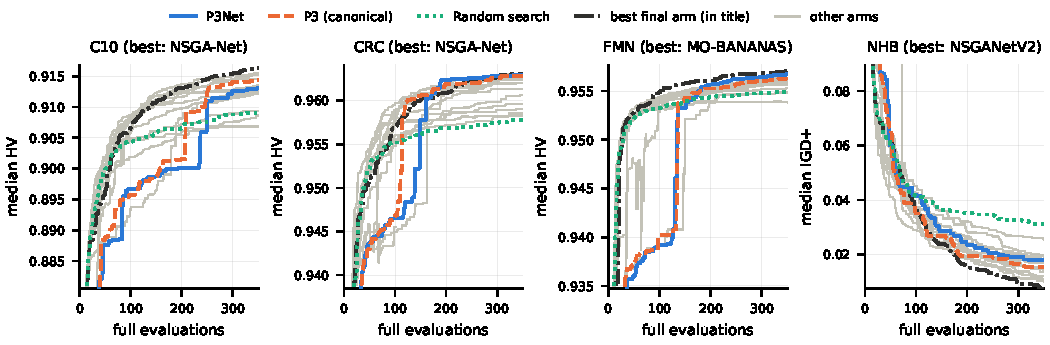
\includegraphics[width=\textwidth]{figures/archive/v005/anytime__primary__budget350.pdf}
    \caption{Anytime quality (pre-registration \S5.1), primary spaces, $b = 350$: median over 30 seeds of the primary metric after each full evaluation (HV higher is better, IGD+ lower is better; y-axis cut to the range after 20 evaluations). Grey: all other main-track arms; dash-dot: the arm with the best median final value in the space. Multi-fidelity arms are on a cost axis and are in the released \texttt{anytime.csv}.}
    \Description{Four line charts, one per primary search space, of median quality against the number of full evaluations up to 350, highlighting P3Net, canonical P3, random search and the best arm.}
    \label{fig:v005-s-anytime}
\end{figure*}
